\documentclass[twoside]{book}

% Packages required by doxygen
\usepackage{fixltx2e}
\usepackage{calc}
\usepackage{doxygen}
\usepackage[export]{adjustbox} % also loads graphicx
\usepackage{graphicx}
\usepackage[utf8]{inputenc}
\usepackage{makeidx}
\usepackage{multicol}
\usepackage{multirow}
\PassOptionsToPackage{warn}{textcomp}
\usepackage{textcomp}
\usepackage[nointegrals]{wasysym}
\usepackage[table]{xcolor}

% Font selection
\usepackage[T1]{fontenc}
\usepackage[scaled=.90]{helvet}
\usepackage{courier}
\usepackage{amssymb}
\usepackage{sectsty}
\renewcommand{\familydefault}{\sfdefault}
\allsectionsfont{%
  \fontseries{bc}\selectfont%
  \color{darkgray}%
}
\renewcommand{\DoxyLabelFont}{%
  \fontseries{bc}\selectfont%
  \color{darkgray}%
}
\newcommand{\+}{\discretionary{\mbox{\scriptsize$\hookleftarrow$}}{}{}}

% Page & text layout
\usepackage{geometry}
\geometry{%
  a4paper,%
  top=2.5cm,%
  bottom=2.5cm,%
  left=2.5cm,%
  right=2.5cm%
}
\tolerance=750
\hfuzz=15pt
\hbadness=750
\setlength{\emergencystretch}{15pt}
\setlength{\parindent}{0cm}
\setlength{\parskip}{3ex plus 2ex minus 2ex}
\makeatletter
\renewcommand{\paragraph}{%
  \@startsection{paragraph}{4}{0ex}{-1.0ex}{1.0ex}{%
    \normalfont\normalsize\bfseries\SS@parafont%
  }%
}
\renewcommand{\subparagraph}{%
  \@startsection{subparagraph}{5}{0ex}{-1.0ex}{1.0ex}{%
    \normalfont\normalsize\bfseries\SS@subparafont%
  }%
}
\makeatother

% Headers & footers
\usepackage{fancyhdr}
\pagestyle{fancyplain}
\fancyhead[LE]{\fancyplain{}{\bfseries\thepage}}
\fancyhead[CE]{\fancyplain{}{}}
\fancyhead[RE]{\fancyplain{}{\bfseries\leftmark}}
\fancyhead[LO]{\fancyplain{}{\bfseries\rightmark}}
\fancyhead[CO]{\fancyplain{}{}}
\fancyhead[RO]{\fancyplain{}{\bfseries\thepage}}
\fancyfoot[LE]{\fancyplain{}{}}
\fancyfoot[CE]{\fancyplain{}{}}
\fancyfoot[RE]{\fancyplain{}{\bfseries\scriptsize Generated by Doxygen }}
\fancyfoot[LO]{\fancyplain{}{\bfseries\scriptsize Generated by Doxygen }}
\fancyfoot[CO]{\fancyplain{}{}}
\fancyfoot[RO]{\fancyplain{}{}}
\renewcommand{\footrulewidth}{0.4pt}
\renewcommand{\chaptermark}[1]{%
  \markboth{#1}{}%
}
\renewcommand{\sectionmark}[1]{%
  \markright{\thesection\ #1}%
}

% Indices & bibliography
\usepackage{natbib}
\usepackage[titles]{tocloft}
\setcounter{tocdepth}{3}
\setcounter{secnumdepth}{5}
\makeindex

% Hyperlinks (required, but should be loaded last)
\usepackage{ifpdf}
\ifpdf
  \usepackage[pdftex,pagebackref=true]{hyperref}
\else
  \usepackage[ps2pdf,pagebackref=true]{hyperref}
\fi
\hypersetup{%
  colorlinks=true,%
  linkcolor=blue,%
  citecolor=blue,%
  unicode%
}

% Custom commands
\newcommand{\clearemptydoublepage}{%
  \newpage{\pagestyle{empty}\cleardoublepage}%
}

\usepackage{caption}
\captionsetup{labelsep=space,justification=centering,font={bf},singlelinecheck=off,skip=4pt,position=top}

%===== C O N T E N T S =====

\begin{document}

% Titlepage & ToC
\hypersetup{pageanchor=false,
             bookmarksnumbered=true,
             pdfencoding=unicode
            }
\pagenumbering{alph}
\begin{titlepage}
\vspace*{7cm}
\begin{center}%
{\Large My Project }\\
\vspace*{1cm}
{\large Generated by Doxygen 1.8.14}\\
\end{center}
\end{titlepage}
\clearemptydoublepage
\pagenumbering{roman}
\tableofcontents
\clearemptydoublepage
\pagenumbering{arabic}
\hypersetup{pageanchor=true}

%--- Begin generated contents ---
\chapter{Hierarchical Index}
\section{Class Hierarchy}
This inheritance list is sorted roughly, but not completely, alphabetically\+:\begin{DoxyCompactList}
\item Base\+Global\+Planner\begin{DoxyCompactList}
\item \contentsline{section}{global\+\_\+planner\+:\+:Global\+Planner}{\pageref{classglobal__planner_1_1_global_planner}}{}
\begin{DoxyCompactList}
\item \contentsline{section}{global\+\_\+planner\+:\+:Planner\+With\+Costmap}{\pageref{classglobal__planner_1_1_planner_with_costmap}}{}
\end{DoxyCompactList}
\end{DoxyCompactList}
\item \contentsline{section}{global\+\_\+planner\+:\+:Expander}{\pageref{classglobal__planner_1_1_expander}}{}
\begin{DoxyCompactList}
\item \contentsline{section}{global\+\_\+planner\+:\+:A\+Star\+Expansion}{\pageref{classglobal__planner_1_1_a_star_expansion}}{}
\item \contentsline{section}{global\+\_\+planner\+:\+:Dijkstra\+Expansion}{\pageref{classglobal__planner_1_1_dijkstra_expansion}}{}
\end{DoxyCompactList}
\item \contentsline{section}{global\+\_\+planner\+:\+:greater1}{\pageref{structglobal__planner_1_1greater1}}{}
\item \contentsline{section}{global\+\_\+planner\+:\+:Index}{\pageref{classglobal__planner_1_1_index}}{}
\item \contentsline{section}{global\+\_\+planner\+:\+:Orientation\+Filter}{\pageref{classglobal__planner_1_1_orientation_filter}}{}
\item \contentsline{section}{Planner\+Core}{\pageref{class_planner_core}}{}
\item \contentsline{section}{global\+\_\+planner\+:\+:Potential\+Calculator}{\pageref{classglobal__planner_1_1_potential_calculator}}{}
\begin{DoxyCompactList}
\item \contentsline{section}{global\+\_\+planner\+:\+:Quadratic\+Calculator}{\pageref{classglobal__planner_1_1_quadratic_calculator}}{}
\end{DoxyCompactList}
\item \contentsline{section}{global\+\_\+planner\+:\+:Traceback}{\pageref{classglobal__planner_1_1_traceback}}{}
\begin{DoxyCompactList}
\item \contentsline{section}{global\+\_\+planner\+:\+:Gradient\+Path}{\pageref{classglobal__planner_1_1_gradient_path}}{}
\item \contentsline{section}{global\+\_\+planner\+:\+:Grid\+Path}{\pageref{classglobal__planner_1_1_grid_path}}{}
\end{DoxyCompactList}
\end{DoxyCompactList}

\chapter{Class Index}
\section{Class List}
Here are the classes, structs, unions and interfaces with brief descriptions\+:\begin{DoxyCompactList}
\item\contentsline{section}{\mbox{\hyperlink{classglobal__planner_1_1_a_star_expansion}{global\+\_\+planner\+::\+A\+Star\+Expansion}} }{\pageref{classglobal__planner_1_1_a_star_expansion}}{}
\item\contentsline{section}{\mbox{\hyperlink{classglobal__planner_1_1_dijkstra_expansion}{global\+\_\+planner\+::\+Dijkstra\+Expansion}} }{\pageref{classglobal__planner_1_1_dijkstra_expansion}}{}
\item\contentsline{section}{\mbox{\hyperlink{classglobal__planner_1_1_expander}{global\+\_\+planner\+::\+Expander}} }{\pageref{classglobal__planner_1_1_expander}}{}
\item\contentsline{section}{\mbox{\hyperlink{classglobal__planner_1_1_global_planner}{global\+\_\+planner\+::\+Global\+Planner}} }{\pageref{classglobal__planner_1_1_global_planner}}{}
\item\contentsline{section}{\mbox{\hyperlink{classglobal__planner_1_1_gradient_path}{global\+\_\+planner\+::\+Gradient\+Path}} }{\pageref{classglobal__planner_1_1_gradient_path}}{}
\item\contentsline{section}{\mbox{\hyperlink{structglobal__planner_1_1greater1}{global\+\_\+planner\+::greater1}} }{\pageref{structglobal__planner_1_1greater1}}{}
\item\contentsline{section}{\mbox{\hyperlink{classglobal__planner_1_1_grid_path}{global\+\_\+planner\+::\+Grid\+Path}} }{\pageref{classglobal__planner_1_1_grid_path}}{}
\item\contentsline{section}{\mbox{\hyperlink{classglobal__planner_1_1_index}{global\+\_\+planner\+::\+Index}} }{\pageref{classglobal__planner_1_1_index}}{}
\item\contentsline{section}{\mbox{\hyperlink{classglobal__planner_1_1_orientation_filter}{global\+\_\+planner\+::\+Orientation\+Filter}} }{\pageref{classglobal__planner_1_1_orientation_filter}}{}
\item\contentsline{section}{\mbox{\hyperlink{class_planner_core}{Planner\+Core}} \\*Provides a R\+OS wrapper for the global\+\_\+planner planner which runs a fast, interpolated navigation function on a costmap }{\pageref{class_planner_core}}{}
\item\contentsline{section}{\mbox{\hyperlink{classglobal__planner_1_1_planner_with_costmap}{global\+\_\+planner\+::\+Planner\+With\+Costmap}} }{\pageref{classglobal__planner_1_1_planner_with_costmap}}{}
\item\contentsline{section}{\mbox{\hyperlink{classglobal__planner_1_1_potential_calculator}{global\+\_\+planner\+::\+Potential\+Calculator}} }{\pageref{classglobal__planner_1_1_potential_calculator}}{}
\item\contentsline{section}{\mbox{\hyperlink{classglobal__planner_1_1_quadratic_calculator}{global\+\_\+planner\+::\+Quadratic\+Calculator}} }{\pageref{classglobal__planner_1_1_quadratic_calculator}}{}
\item\contentsline{section}{\mbox{\hyperlink{classglobal__planner_1_1_traceback}{global\+\_\+planner\+::\+Traceback}} }{\pageref{classglobal__planner_1_1_traceback}}{}
\end{DoxyCompactList}

\chapter{Class Documentation}
\hypertarget{classglobal__planner_1_1_a_star_expansion}{}\section{global\+\_\+planner\+:\+:A\+Star\+Expansion Class Reference}
\label{classglobal__planner_1_1_a_star_expansion}\index{global\+\_\+planner\+::\+A\+Star\+Expansion@{global\+\_\+planner\+::\+A\+Star\+Expansion}}
Inheritance diagram for global\+\_\+planner\+:\+:A\+Star\+Expansion\+:\begin{figure}[H]
\begin{center}
\leavevmode
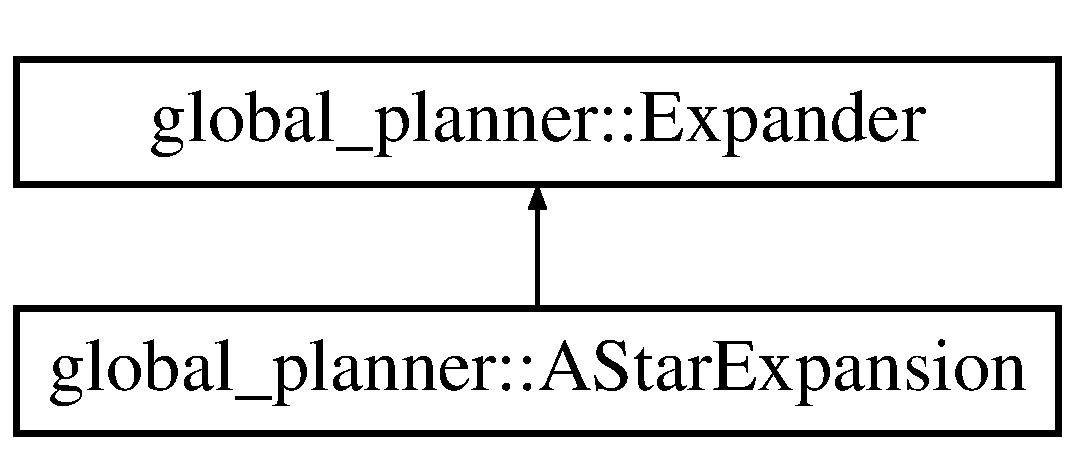
\includegraphics[height=2.000000cm]{classglobal__planner_1_1_a_star_expansion}
\end{center}
\end{figure}
\subsection*{Public Member Functions}
\begin{DoxyCompactItemize}
\item 
\mbox{\Hypertarget{classglobal__planner_1_1_a_star_expansion_a3a1f2f9b946d0e69afce5886cf7d56fa}\label{classglobal__planner_1_1_a_star_expansion_a3a1f2f9b946d0e69afce5886cf7d56fa}} 
{\bfseries A\+Star\+Expansion} (\mbox{\hyperlink{classglobal__planner_1_1_potential_calculator}{Potential\+Calculator}} $\ast$p\+\_\+calc, int nx, int ny)
\item 
\mbox{\Hypertarget{classglobal__planner_1_1_a_star_expansion_a71ddf1440a2f487c6f10af7a25757371}\label{classglobal__planner_1_1_a_star_expansion_a71ddf1440a2f487c6f10af7a25757371}} 
bool {\bfseries calculate\+Potentials} (unsigned char $\ast$costs, double start\+\_\+x, double start\+\_\+y, double end\+\_\+x, double end\+\_\+y, int cycles, float $\ast$potential)
\end{DoxyCompactItemize}
\subsection*{Additional Inherited Members}


The documentation for this class was generated from the following files\+:\begin{DoxyCompactItemize}
\item 
include/global\+\_\+planner/astar.\+h\item 
src/astar.\+cpp\end{DoxyCompactItemize}

\hypertarget{classglobal__planner_1_1_dijkstra_expansion}{}\section{global\+\_\+planner\+:\+:Dijkstra\+Expansion Class Reference}
\label{classglobal__planner_1_1_dijkstra_expansion}\index{global\+\_\+planner\+::\+Dijkstra\+Expansion@{global\+\_\+planner\+::\+Dijkstra\+Expansion}}
Inheritance diagram for global\+\_\+planner\+:\+:Dijkstra\+Expansion\+:\begin{figure}[H]
\begin{center}
\leavevmode
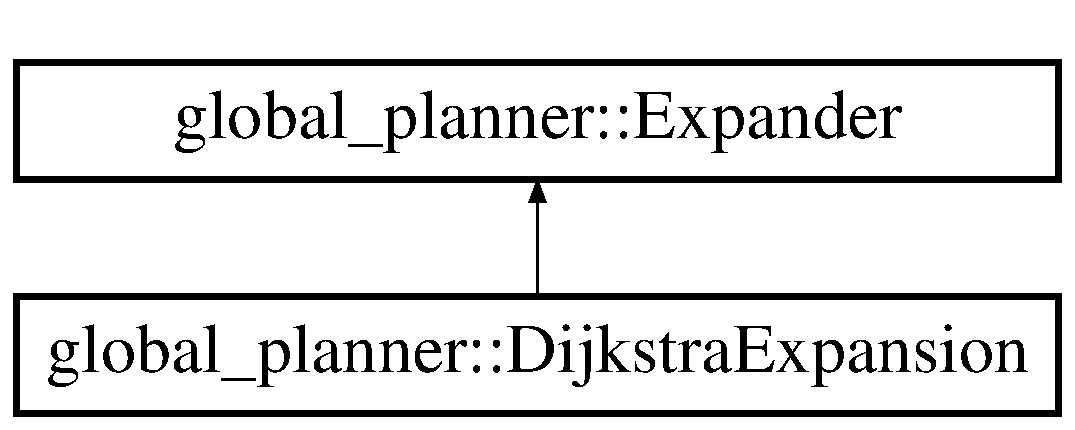
\includegraphics[height=2.000000cm]{classglobal__planner_1_1_dijkstra_expansion}
\end{center}
\end{figure}
\subsection*{Public Member Functions}
\begin{DoxyCompactItemize}
\item 
\mbox{\Hypertarget{classglobal__planner_1_1_dijkstra_expansion_a58e6885deccbdab45ecda172bb74c702}\label{classglobal__planner_1_1_dijkstra_expansion_a58e6885deccbdab45ecda172bb74c702}} 
{\bfseries Dijkstra\+Expansion} (\mbox{\hyperlink{classglobal__planner_1_1_potential_calculator}{Potential\+Calculator}} $\ast$p\+\_\+calc, int nx, int ny)
\item 
\mbox{\Hypertarget{classglobal__planner_1_1_dijkstra_expansion_a1102e169bb79dac31de8fe5ca5ace39b}\label{classglobal__planner_1_1_dijkstra_expansion_a1102e169bb79dac31de8fe5ca5ace39b}} 
bool {\bfseries calculate\+Potentials} (unsigned char $\ast$costs, double start\+\_\+x, double start\+\_\+y, double end\+\_\+x, double end\+\_\+y, int cycles, float $\ast$potential)
\item 
void \mbox{\hyperlink{classglobal__planner_1_1_dijkstra_expansion_a7d286126b2c478fc55c5e995e1deff29}{set\+Size}} (int nx, int ny)
\begin{DoxyCompactList}\small\item\em Sets or resets the size of the map. \end{DoxyCompactList}\item 
\mbox{\Hypertarget{classglobal__planner_1_1_dijkstra_expansion_a2ec5a9b73f4a8680adc8e406bc18b254}\label{classglobal__planner_1_1_dijkstra_expansion_a2ec5a9b73f4a8680adc8e406bc18b254}} 
void {\bfseries set\+Neutral\+Cost} (unsigned char neutral\+\_\+cost)
\item 
\mbox{\Hypertarget{classglobal__planner_1_1_dijkstra_expansion_a5ba5aa2bff86fd1b18b24163379d9e2b}\label{classglobal__planner_1_1_dijkstra_expansion_a5ba5aa2bff86fd1b18b24163379d9e2b}} 
void {\bfseries set\+Precise\+Start} (bool precise)
\end{DoxyCompactItemize}
\subsection*{Additional Inherited Members}


\subsection{Member Function Documentation}
\mbox{\Hypertarget{classglobal__planner_1_1_dijkstra_expansion_a7d286126b2c478fc55c5e995e1deff29}\label{classglobal__planner_1_1_dijkstra_expansion_a7d286126b2c478fc55c5e995e1deff29}} 
\index{global\+\_\+planner\+::\+Dijkstra\+Expansion@{global\+\_\+planner\+::\+Dijkstra\+Expansion}!set\+Size@{set\+Size}}
\index{set\+Size@{set\+Size}!global\+\_\+planner\+::\+Dijkstra\+Expansion@{global\+\_\+planner\+::\+Dijkstra\+Expansion}}
\subsubsection{\texorpdfstring{set\+Size()}{setSize()}}
{\footnotesize\ttfamily void global\+\_\+planner\+::\+Dijkstra\+Expansion\+::set\+Size (\begin{DoxyParamCaption}\item[{int}]{nx,  }\item[{int}]{ny }\end{DoxyParamCaption})\hspace{0.3cm}{\ttfamily [virtual]}}



Sets or resets the size of the map. 


\begin{DoxyParams}{Parameters}
{\em nx} & The x size of the map \\
\hline
{\em ny} & The y size of the mapsets or resets the size of the map \\
\hline
\end{DoxyParams}


Reimplemented from \mbox{\hyperlink{classglobal__planner_1_1_expander_aeeaa60103de1ee71a1969e40a3735094}{global\+\_\+planner\+::\+Expander}}.



The documentation for this class was generated from the following files\+:\begin{DoxyCompactItemize}
\item 
include/global\+\_\+planner/dijkstra.\+h\item 
src/dijkstra.\+cpp\end{DoxyCompactItemize}

\hypertarget{classglobal__planner_1_1_expander}{}\section{global\+\_\+planner\+:\+:Expander Class Reference}
\label{classglobal__planner_1_1_expander}\index{global\+\_\+planner\+::\+Expander@{global\+\_\+planner\+::\+Expander}}
Inheritance diagram for global\+\_\+planner\+:\+:Expander\+:\begin{figure}[H]
\begin{center}
\leavevmode
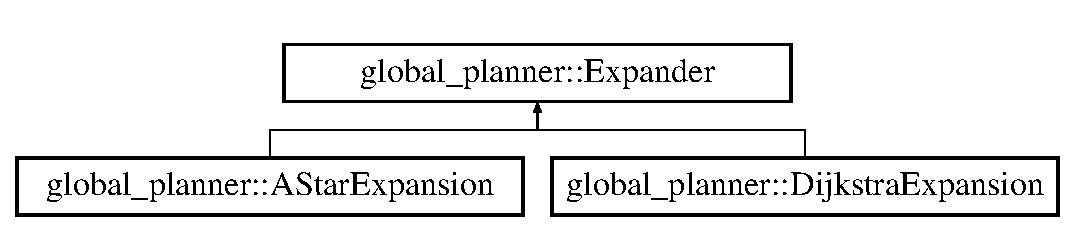
\includegraphics[height=2.000000cm]{classglobal__planner_1_1_expander}
\end{center}
\end{figure}
\subsection*{Public Member Functions}
\begin{DoxyCompactItemize}
\item 
\mbox{\Hypertarget{classglobal__planner_1_1_expander_a8ccb306a28ea41d2bfd9202d4b16f26a}\label{classglobal__planner_1_1_expander_a8ccb306a28ea41d2bfd9202d4b16f26a}} 
{\bfseries Expander} (\mbox{\hyperlink{classglobal__planner_1_1_potential_calculator}{Potential\+Calculator}} $\ast$p\+\_\+calc, int nx, int ny)
\item 
\mbox{\Hypertarget{classglobal__planner_1_1_expander_a7c352121a2ea1e1b650b219004c98786}\label{classglobal__planner_1_1_expander_a7c352121a2ea1e1b650b219004c98786}} 
virtual bool {\bfseries calculate\+Potentials} (unsigned char $\ast$costs, double start\+\_\+x, double start\+\_\+y, double end\+\_\+x, double end\+\_\+y, int cycles, float $\ast$potential)=0
\item 
virtual void \mbox{\hyperlink{classglobal__planner_1_1_expander_aeeaa60103de1ee71a1969e40a3735094}{set\+Size}} (int nx, int ny)
\begin{DoxyCompactList}\small\item\em Sets or resets the size of the map. \end{DoxyCompactList}\item 
\mbox{\Hypertarget{classglobal__planner_1_1_expander_aee9c360fb6316c538bbadcccc6bf98b1}\label{classglobal__planner_1_1_expander_aee9c360fb6316c538bbadcccc6bf98b1}} 
void {\bfseries set\+Lethal\+Cost} (unsigned char lethal\+\_\+cost)
\item 
\mbox{\Hypertarget{classglobal__planner_1_1_expander_a386d3239f3aaa7a5e583bad9893a8ca1}\label{classglobal__planner_1_1_expander_a386d3239f3aaa7a5e583bad9893a8ca1}} 
void {\bfseries set\+Neutral\+Cost} (unsigned char neutral\+\_\+cost)
\item 
\mbox{\Hypertarget{classglobal__planner_1_1_expander_a53a3174aef024f0a4d01ac3fa7a74489}\label{classglobal__planner_1_1_expander_a53a3174aef024f0a4d01ac3fa7a74489}} 
void {\bfseries set\+Factor} (float factor)
\item 
\mbox{\Hypertarget{classglobal__planner_1_1_expander_a1dcbac968719e195552d063c4314618e}\label{classglobal__planner_1_1_expander_a1dcbac968719e195552d063c4314618e}} 
void {\bfseries set\+Has\+Unknown} (bool unknown)
\item 
\mbox{\Hypertarget{classglobal__planner_1_1_expander_a02060106b60c2661cb1f1878a151a40e}\label{classglobal__planner_1_1_expander_a02060106b60c2661cb1f1878a151a40e}} 
void {\bfseries clear\+Endpoint} (unsigned char $\ast$costs, float $\ast$potential, int gx, int gy, int s)
\end{DoxyCompactItemize}
\subsection*{Protected Member Functions}
\begin{DoxyCompactItemize}
\item 
\mbox{\Hypertarget{classglobal__planner_1_1_expander_ab9ed0e500049774014960dfb68f1e50c}\label{classglobal__planner_1_1_expander_ab9ed0e500049774014960dfb68f1e50c}} 
int {\bfseries to\+Index} (int x, int y)
\end{DoxyCompactItemize}
\subsection*{Protected Attributes}
\begin{DoxyCompactItemize}
\item 
\mbox{\Hypertarget{classglobal__planner_1_1_expander_a72bbafddd4f838603ebe42cf7fb57cbc}\label{classglobal__planner_1_1_expander_a72bbafddd4f838603ebe42cf7fb57cbc}} 
int {\bfseries nx\+\_\+}
\item 
\mbox{\Hypertarget{classglobal__planner_1_1_expander_a3d1877778a6ed03533dace263d0dbe7e}\label{classglobal__planner_1_1_expander_a3d1877778a6ed03533dace263d0dbe7e}} 
int {\bfseries ny\+\_\+}
\item 
int \mbox{\hyperlink{classglobal__planner_1_1_expander_a0538b977e9cd0022810096b79e61e529}{ns\+\_\+}}
\item 
\mbox{\Hypertarget{classglobal__planner_1_1_expander_abbb2fc0fd78f4ae3e8ffad2981629a91}\label{classglobal__planner_1_1_expander_abbb2fc0fd78f4ae3e8ffad2981629a91}} 
bool {\bfseries unknown\+\_\+}
\item 
\mbox{\Hypertarget{classglobal__planner_1_1_expander_a044a34d5d5ddd41016afec643cb65d4e}\label{classglobal__planner_1_1_expander_a044a34d5d5ddd41016afec643cb65d4e}} 
unsigned char {\bfseries lethal\+\_\+cost\+\_\+}
\item 
\mbox{\Hypertarget{classglobal__planner_1_1_expander_aa8941c07a0f50a2e3ce3088f7ecb8e61}\label{classglobal__planner_1_1_expander_aa8941c07a0f50a2e3ce3088f7ecb8e61}} 
unsigned char {\bfseries neutral\+\_\+cost\+\_\+}
\item 
\mbox{\Hypertarget{classglobal__planner_1_1_expander_ad51bd3f97e8d1ca48c357175d723f3f4}\label{classglobal__planner_1_1_expander_ad51bd3f97e8d1ca48c357175d723f3f4}} 
int {\bfseries cells\+\_\+visited\+\_\+}
\item 
\mbox{\Hypertarget{classglobal__planner_1_1_expander_a999123a5d229a31933a64ba56a4f525d}\label{classglobal__planner_1_1_expander_a999123a5d229a31933a64ba56a4f525d}} 
float {\bfseries factor\+\_\+}
\item 
\mbox{\Hypertarget{classglobal__planner_1_1_expander_a3d991703be557e08056daedd3d872fff}\label{classglobal__planner_1_1_expander_a3d991703be557e08056daedd3d872fff}} 
\mbox{\hyperlink{classglobal__planner_1_1_potential_calculator}{Potential\+Calculator}} $\ast$ {\bfseries p\+\_\+calc\+\_\+}
\end{DoxyCompactItemize}


\subsection{Member Function Documentation}
\mbox{\Hypertarget{classglobal__planner_1_1_expander_aeeaa60103de1ee71a1969e40a3735094}\label{classglobal__planner_1_1_expander_aeeaa60103de1ee71a1969e40a3735094}} 
\index{global\+\_\+planner\+::\+Expander@{global\+\_\+planner\+::\+Expander}!set\+Size@{set\+Size}}
\index{set\+Size@{set\+Size}!global\+\_\+planner\+::\+Expander@{global\+\_\+planner\+::\+Expander}}
\subsubsection{\texorpdfstring{set\+Size()}{setSize()}}
{\footnotesize\ttfamily virtual void global\+\_\+planner\+::\+Expander\+::set\+Size (\begin{DoxyParamCaption}\item[{int}]{nx,  }\item[{int}]{ny }\end{DoxyParamCaption})\hspace{0.3cm}{\ttfamily [inline]}, {\ttfamily [virtual]}}



Sets or resets the size of the map. 


\begin{DoxyParams}{Parameters}
{\em nx} & The x size of the map \\
\hline
{\em ny} & The y size of the mapsets or resets the size of the map \\
\hline
\end{DoxyParams}


Reimplemented in \mbox{\hyperlink{classglobal__planner_1_1_dijkstra_expansion_a7d286126b2c478fc55c5e995e1deff29}{global\+\_\+planner\+::\+Dijkstra\+Expansion}}.



\subsection{Member Data Documentation}
\mbox{\Hypertarget{classglobal__planner_1_1_expander_a0538b977e9cd0022810096b79e61e529}\label{classglobal__planner_1_1_expander_a0538b977e9cd0022810096b79e61e529}} 
\index{global\+\_\+planner\+::\+Expander@{global\+\_\+planner\+::\+Expander}!ns\+\_\+@{ns\+\_\+}}
\index{ns\+\_\+@{ns\+\_\+}!global\+\_\+planner\+::\+Expander@{global\+\_\+planner\+::\+Expander}}
\subsubsection{\texorpdfstring{ns\+\_\+}{ns\_}}
{\footnotesize\ttfamily int global\+\_\+planner\+::\+Expander\+::ns\+\_\+\hspace{0.3cm}{\ttfamily [protected]}}

size of grid, in pixels 

The documentation for this class was generated from the following file\+:\begin{DoxyCompactItemize}
\item 
include/global\+\_\+planner/expander.\+h\end{DoxyCompactItemize}

\hypertarget{classglobal__planner_1_1_global_planner}{}\section{global\+\_\+planner\+:\+:Global\+Planner Class Reference}
\label{classglobal__planner_1_1_global_planner}\index{global\+\_\+planner\+::\+Global\+Planner@{global\+\_\+planner\+::\+Global\+Planner}}
Inheritance diagram for global\+\_\+planner\+:\+:Global\+Planner\+:\begin{figure}[H]
\begin{center}
\leavevmode
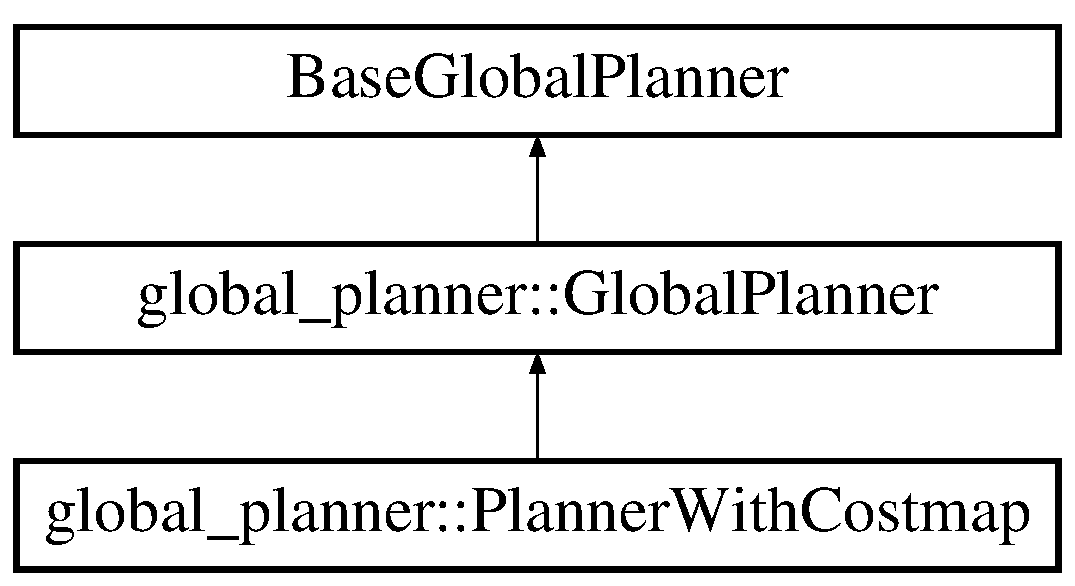
\includegraphics[height=3.000000cm]{classglobal__planner_1_1_global_planner}
\end{center}
\end{figure}
\subsection*{Public Member Functions}
\begin{DoxyCompactItemize}
\item 
\mbox{\Hypertarget{classglobal__planner_1_1_global_planner_a69b66f59b51665f826a51587afa720ff}\label{classglobal__planner_1_1_global_planner_a69b66f59b51665f826a51587afa720ff}} 
\mbox{\hyperlink{classglobal__planner_1_1_global_planner_a69b66f59b51665f826a51587afa720ff}{Global\+Planner}} ()
\begin{DoxyCompactList}\small\item\em Default constructor for the \mbox{\hyperlink{class_planner_core}{Planner\+Core}} object. \end{DoxyCompactList}\item 
\mbox{\hyperlink{classglobal__planner_1_1_global_planner_aaeb34983765b053861cbef08e9614bb5}{Global\+Planner}} (std\+::string name, costmap\+\_\+2d\+::\+Costmap2D $\ast$costmap, std\+::string frame\+\_\+id)
\begin{DoxyCompactList}\small\item\em Constructor for the \mbox{\hyperlink{class_planner_core}{Planner\+Core}} object. \end{DoxyCompactList}\item 
\mbox{\Hypertarget{classglobal__planner_1_1_global_planner_aa49ab75794afdbec6aa7c6c3902de4c0}\label{classglobal__planner_1_1_global_planner_aa49ab75794afdbec6aa7c6c3902de4c0}} 
\mbox{\hyperlink{classglobal__planner_1_1_global_planner_aa49ab75794afdbec6aa7c6c3902de4c0}{$\sim$\+Global\+Planner}} ()
\begin{DoxyCompactList}\small\item\em Default deconstructor for the \mbox{\hyperlink{class_planner_core}{Planner\+Core}} object. \end{DoxyCompactList}\item 
void \mbox{\hyperlink{classglobal__planner_1_1_global_planner_a280ebb6723d46b462eb66ec73a2fe266}{initialize}} (std\+::string name, costmap\+\_\+2d\+::\+Costmap2\+D\+R\+OS $\ast$costmap\+\_\+ros)
\begin{DoxyCompactList}\small\item\em Initialization function for the \mbox{\hyperlink{class_planner_core}{Planner\+Core}} object. \end{DoxyCompactList}\item 
\mbox{\Hypertarget{classglobal__planner_1_1_global_planner_af3ade8f9f487fe2ddd109f0845a6ffb2}\label{classglobal__planner_1_1_global_planner_af3ade8f9f487fe2ddd109f0845a6ffb2}} 
void {\bfseries initialize} (std\+::string name, costmap\+\_\+2d\+::\+Costmap2D $\ast$costmap, std\+::string frame\+\_\+id)
\item 
bool \mbox{\hyperlink{classglobal__planner_1_1_global_planner_abb7f40f6a851f88e6b7668a38571712a}{make\+Plan}} (const geometry\+\_\+msgs\+::\+Pose\+Stamped \&start, const geometry\+\_\+msgs\+::\+Pose\+Stamped \&goal, std\+::vector$<$ geometry\+\_\+msgs\+::\+Pose\+Stamped $>$ \&plan)
\begin{DoxyCompactList}\small\item\em Given a goal pose in the world, compute a plan. \end{DoxyCompactList}\item 
bool \mbox{\hyperlink{classglobal__planner_1_1_global_planner_a4f6bfa5acf58670c01a5b8c684a2f20c}{make\+Plan}} (const geometry\+\_\+msgs\+::\+Pose\+Stamped \&start, const geometry\+\_\+msgs\+::\+Pose\+Stamped \&goal, double tolerance, std\+::vector$<$ geometry\+\_\+msgs\+::\+Pose\+Stamped $>$ \&plan)
\begin{DoxyCompactList}\small\item\em Given a goal pose in the world, compute a plan. \end{DoxyCompactList}\item 
bool \mbox{\hyperlink{classglobal__planner_1_1_global_planner_aa64e1114c4a78980256bd04bd0e79efa}{compute\+Potential}} (const geometry\+\_\+msgs\+::\+Point \&world\+\_\+point)
\begin{DoxyCompactList}\small\item\em Computes the full navigation function for the map given a point in the world to start from. \end{DoxyCompactList}\item 
bool \mbox{\hyperlink{classglobal__planner_1_1_global_planner_a4bae9ef237ecc53aa3027abd3dc063b5}{get\+Plan\+From\+Potential}} (double start\+\_\+x, double start\+\_\+y, double end\+\_\+x, double end\+\_\+y, const geometry\+\_\+msgs\+::\+Pose\+Stamped \&goal, std\+::vector$<$ geometry\+\_\+msgs\+::\+Pose\+Stamped $>$ \&plan)
\begin{DoxyCompactList}\small\item\em Compute a plan to a goal after the potential for a start point has already been computed (Note\+: You should call compute\+Potential first) \end{DoxyCompactList}\item 
double \mbox{\hyperlink{classglobal__planner_1_1_global_planner_a7f0a8eaf0e715f682480ef447a63cd67}{get\+Point\+Potential}} (const geometry\+\_\+msgs\+::\+Point \&world\+\_\+point)
\begin{DoxyCompactList}\small\item\em Get the potential, or naviagation cost, at a given point in the world (Note\+: You should call compute\+Potential first) \end{DoxyCompactList}\item 
bool \mbox{\hyperlink{classglobal__planner_1_1_global_planner_a7c50827ebb21a48825d55bda56dd38ac}{valid\+Point\+Potential}} (const geometry\+\_\+msgs\+::\+Point \&world\+\_\+point)
\begin{DoxyCompactList}\small\item\em Check for a valid potential value at a given point in the world (Note\+: You should call compute\+Potential first) \end{DoxyCompactList}\item 
bool \mbox{\hyperlink{classglobal__planner_1_1_global_planner_a27405d9450075e6dcc7fc73bd56fb6dc}{valid\+Point\+Potential}} (const geometry\+\_\+msgs\+::\+Point \&world\+\_\+point, double tolerance)
\begin{DoxyCompactList}\small\item\em Check for a valid potential value at a given point in the world (Note\+: You should call compute\+Potential first) \end{DoxyCompactList}\item 
\mbox{\Hypertarget{classglobal__planner_1_1_global_planner_a9844153b2bea9032522a2ed528be963f}\label{classglobal__planner_1_1_global_planner_a9844153b2bea9032522a2ed528be963f}} 
void \mbox{\hyperlink{classglobal__planner_1_1_global_planner_a9844153b2bea9032522a2ed528be963f}{publish\+Plan}} (const std\+::vector$<$ geometry\+\_\+msgs\+::\+Pose\+Stamped $>$ \&path)
\begin{DoxyCompactList}\small\item\em Publish a path for visualization purposes. \end{DoxyCompactList}\item 
\mbox{\Hypertarget{classglobal__planner_1_1_global_planner_a760dc206a99babddfacded0558d35208}\label{classglobal__planner_1_1_global_planner_a760dc206a99babddfacded0558d35208}} 
bool {\bfseries make\+Plan\+Service} (nav\+\_\+msgs\+::\+Get\+Plan\+::\+Request \&req, nav\+\_\+msgs\+::\+Get\+Plan\+::\+Response \&resp)
\end{DoxyCompactItemize}
\subsection*{Protected Attributes}
\begin{DoxyCompactItemize}
\item 
\mbox{\Hypertarget{classglobal__planner_1_1_global_planner_a790fb19fb46e1a1edc15f98b1075e849}\label{classglobal__planner_1_1_global_planner_a790fb19fb46e1a1edc15f98b1075e849}} 
costmap\+\_\+2d\+::\+Costmap2D $\ast$ \mbox{\hyperlink{classglobal__planner_1_1_global_planner_a790fb19fb46e1a1edc15f98b1075e849}{costmap\+\_\+}}
\begin{DoxyCompactList}\small\item\em Store a copy of the current costmap in {\itshape costmap}. Called by make\+Plan. \end{DoxyCompactList}\item 
\mbox{\Hypertarget{classglobal__planner_1_1_global_planner_a4a8bf49e32dcae69b02adabe35b99ed0}\label{classglobal__planner_1_1_global_planner_a4a8bf49e32dcae69b02adabe35b99ed0}} 
std\+::string {\bfseries frame\+\_\+id\+\_\+}
\item 
\mbox{\Hypertarget{classglobal__planner_1_1_global_planner_ae90f4043291a203f62ad9259796792dc}\label{classglobal__planner_1_1_global_planner_ae90f4043291a203f62ad9259796792dc}} 
ros\+::\+Publisher {\bfseries plan\+\_\+pub\+\_\+}
\item 
\mbox{\Hypertarget{classglobal__planner_1_1_global_planner_abd54fe2b4a6f92fec92e49da3739e016}\label{classglobal__planner_1_1_global_planner_abd54fe2b4a6f92fec92e49da3739e016}} 
bool {\bfseries initialized\+\_\+}
\item 
\mbox{\Hypertarget{classglobal__planner_1_1_global_planner_adc356fbcaa27c897710becc5f7ad9777}\label{classglobal__planner_1_1_global_planner_adc356fbcaa27c897710becc5f7ad9777}} 
bool {\bfseries allow\+\_\+unknown\+\_\+}
\item 
\mbox{\Hypertarget{classglobal__planner_1_1_global_planner_a74d3e7b867447cea6d718350fc0b303b}\label{classglobal__planner_1_1_global_planner_a74d3e7b867447cea6d718350fc0b303b}} 
bool {\bfseries visualize\+\_\+potential\+\_\+}
\end{DoxyCompactItemize}


\subsection{Constructor \& Destructor Documentation}
\mbox{\Hypertarget{classglobal__planner_1_1_global_planner_aaeb34983765b053861cbef08e9614bb5}\label{classglobal__planner_1_1_global_planner_aaeb34983765b053861cbef08e9614bb5}} 
\index{global\+\_\+planner\+::\+Global\+Planner@{global\+\_\+planner\+::\+Global\+Planner}!Global\+Planner@{Global\+Planner}}
\index{Global\+Planner@{Global\+Planner}!global\+\_\+planner\+::\+Global\+Planner@{global\+\_\+planner\+::\+Global\+Planner}}
\subsubsection{\texorpdfstring{Global\+Planner()}{GlobalPlanner()}}
{\footnotesize\ttfamily global\+\_\+planner\+::\+Global\+Planner\+::\+Global\+Planner (\begin{DoxyParamCaption}\item[{std\+::string}]{name,  }\item[{costmap\+\_\+2d\+::\+Costmap2D $\ast$}]{costmap,  }\item[{std\+::string}]{frame\+\_\+id }\end{DoxyParamCaption})}



Constructor for the \mbox{\hyperlink{class_planner_core}{Planner\+Core}} object. 


\begin{DoxyParams}{Parameters}
{\em name} & The name of this planner \\
\hline
{\em costmap} & A pointer to the costmap to use \\
\hline
{\em frame\+\_\+id} & Frame of the costmap \\
\hline
\end{DoxyParams}


\subsection{Member Function Documentation}
\mbox{\Hypertarget{classglobal__planner_1_1_global_planner_aa64e1114c4a78980256bd04bd0e79efa}\label{classglobal__planner_1_1_global_planner_aa64e1114c4a78980256bd04bd0e79efa}} 
\index{global\+\_\+planner\+::\+Global\+Planner@{global\+\_\+planner\+::\+Global\+Planner}!compute\+Potential@{compute\+Potential}}
\index{compute\+Potential@{compute\+Potential}!global\+\_\+planner\+::\+Global\+Planner@{global\+\_\+planner\+::\+Global\+Planner}}
\subsubsection{\texorpdfstring{compute\+Potential()}{computePotential()}}
{\footnotesize\ttfamily bool global\+\_\+planner\+::\+Global\+Planner\+::compute\+Potential (\begin{DoxyParamCaption}\item[{const geometry\+\_\+msgs\+::\+Point \&}]{world\+\_\+point }\end{DoxyParamCaption})}



Computes the full navigation function for the map given a point in the world to start from. 


\begin{DoxyParams}{Parameters}
{\em world\+\_\+point} & The point to use for seeding the navigation function \\
\hline
\end{DoxyParams}
\begin{DoxyReturn}{Returns}
True if the navigation function was computed successfully, false otherwise 
\end{DoxyReturn}
\mbox{\Hypertarget{classglobal__planner_1_1_global_planner_a4bae9ef237ecc53aa3027abd3dc063b5}\label{classglobal__planner_1_1_global_planner_a4bae9ef237ecc53aa3027abd3dc063b5}} 
\index{global\+\_\+planner\+::\+Global\+Planner@{global\+\_\+planner\+::\+Global\+Planner}!get\+Plan\+From\+Potential@{get\+Plan\+From\+Potential}}
\index{get\+Plan\+From\+Potential@{get\+Plan\+From\+Potential}!global\+\_\+planner\+::\+Global\+Planner@{global\+\_\+planner\+::\+Global\+Planner}}
\subsubsection{\texorpdfstring{get\+Plan\+From\+Potential()}{getPlanFromPotential()}}
{\footnotesize\ttfamily bool global\+\_\+planner\+::\+Global\+Planner\+::get\+Plan\+From\+Potential (\begin{DoxyParamCaption}\item[{double}]{start\+\_\+x,  }\item[{double}]{start\+\_\+y,  }\item[{double}]{end\+\_\+x,  }\item[{double}]{end\+\_\+y,  }\item[{const geometry\+\_\+msgs\+::\+Pose\+Stamped \&}]{goal,  }\item[{std\+::vector$<$ geometry\+\_\+msgs\+::\+Pose\+Stamped $>$ \&}]{plan }\end{DoxyParamCaption})}



Compute a plan to a goal after the potential for a start point has already been computed (Note\+: You should call compute\+Potential first) 


\begin{DoxyParams}{Parameters}
{\em start\+\_\+x} & \\
\hline
{\em start\+\_\+y} & \\
\hline
{\em end\+\_\+x} & \\
\hline
{\em end\+\_\+y} & \\
\hline
{\em goal} & The goal pose to create a plan to \\
\hline
{\em plan} & The plan... filled by the planner \\
\hline
\end{DoxyParams}
\begin{DoxyReturn}{Returns}
True if a valid plan was found, false otherwise 
\end{DoxyReturn}
\mbox{\Hypertarget{classglobal__planner_1_1_global_planner_a7f0a8eaf0e715f682480ef447a63cd67}\label{classglobal__planner_1_1_global_planner_a7f0a8eaf0e715f682480ef447a63cd67}} 
\index{global\+\_\+planner\+::\+Global\+Planner@{global\+\_\+planner\+::\+Global\+Planner}!get\+Point\+Potential@{get\+Point\+Potential}}
\index{get\+Point\+Potential@{get\+Point\+Potential}!global\+\_\+planner\+::\+Global\+Planner@{global\+\_\+planner\+::\+Global\+Planner}}
\subsubsection{\texorpdfstring{get\+Point\+Potential()}{getPointPotential()}}
{\footnotesize\ttfamily double global\+\_\+planner\+::\+Global\+Planner\+::get\+Point\+Potential (\begin{DoxyParamCaption}\item[{const geometry\+\_\+msgs\+::\+Point \&}]{world\+\_\+point }\end{DoxyParamCaption})}



Get the potential, or naviagation cost, at a given point in the world (Note\+: You should call compute\+Potential first) 


\begin{DoxyParams}{Parameters}
{\em world\+\_\+point} & The point to get the potential for \\
\hline
\end{DoxyParams}
\begin{DoxyReturn}{Returns}
The navigation function\textquotesingle{}s value at that point in the world 
\end{DoxyReturn}
\mbox{\Hypertarget{classglobal__planner_1_1_global_planner_a280ebb6723d46b462eb66ec73a2fe266}\label{classglobal__planner_1_1_global_planner_a280ebb6723d46b462eb66ec73a2fe266}} 
\index{global\+\_\+planner\+::\+Global\+Planner@{global\+\_\+planner\+::\+Global\+Planner}!initialize@{initialize}}
\index{initialize@{initialize}!global\+\_\+planner\+::\+Global\+Planner@{global\+\_\+planner\+::\+Global\+Planner}}
\subsubsection{\texorpdfstring{initialize()}{initialize()}}
{\footnotesize\ttfamily void global\+\_\+planner\+::\+Global\+Planner\+::initialize (\begin{DoxyParamCaption}\item[{std\+::string}]{name,  }\item[{costmap\+\_\+2d\+::\+Costmap2\+D\+R\+OS $\ast$}]{costmap\+\_\+ros }\end{DoxyParamCaption})}



Initialization function for the \mbox{\hyperlink{class_planner_core}{Planner\+Core}} object. 


\begin{DoxyParams}{Parameters}
{\em name} & The name of this planner \\
\hline
{\em costmap\+\_\+ros} & A pointer to the R\+OS wrapper of the costmap to use for planning \\
\hline
\end{DoxyParams}
\mbox{\Hypertarget{classglobal__planner_1_1_global_planner_abb7f40f6a851f88e6b7668a38571712a}\label{classglobal__planner_1_1_global_planner_abb7f40f6a851f88e6b7668a38571712a}} 
\index{global\+\_\+planner\+::\+Global\+Planner@{global\+\_\+planner\+::\+Global\+Planner}!make\+Plan@{make\+Plan}}
\index{make\+Plan@{make\+Plan}!global\+\_\+planner\+::\+Global\+Planner@{global\+\_\+planner\+::\+Global\+Planner}}
\subsubsection{\texorpdfstring{make\+Plan()}{makePlan()}\hspace{0.1cm}{\footnotesize\ttfamily [1/2]}}
{\footnotesize\ttfamily bool global\+\_\+planner\+::\+Global\+Planner\+::make\+Plan (\begin{DoxyParamCaption}\item[{const geometry\+\_\+msgs\+::\+Pose\+Stamped \&}]{start,  }\item[{const geometry\+\_\+msgs\+::\+Pose\+Stamped \&}]{goal,  }\item[{std\+::vector$<$ geometry\+\_\+msgs\+::\+Pose\+Stamped $>$ \&}]{plan }\end{DoxyParamCaption})}



Given a goal pose in the world, compute a plan. 


\begin{DoxyParams}{Parameters}
{\em start} & The start pose \\
\hline
{\em goal} & The goal pose \\
\hline
{\em plan} & The plan... filled by the planner \\
\hline
\end{DoxyParams}
\begin{DoxyReturn}{Returns}
True if a valid plan was found, false otherwise 
\end{DoxyReturn}
\mbox{\Hypertarget{classglobal__planner_1_1_global_planner_a4f6bfa5acf58670c01a5b8c684a2f20c}\label{classglobal__planner_1_1_global_planner_a4f6bfa5acf58670c01a5b8c684a2f20c}} 
\index{global\+\_\+planner\+::\+Global\+Planner@{global\+\_\+planner\+::\+Global\+Planner}!make\+Plan@{make\+Plan}}
\index{make\+Plan@{make\+Plan}!global\+\_\+planner\+::\+Global\+Planner@{global\+\_\+planner\+::\+Global\+Planner}}
\subsubsection{\texorpdfstring{make\+Plan()}{makePlan()}\hspace{0.1cm}{\footnotesize\ttfamily [2/2]}}
{\footnotesize\ttfamily bool global\+\_\+planner\+::\+Global\+Planner\+::make\+Plan (\begin{DoxyParamCaption}\item[{const geometry\+\_\+msgs\+::\+Pose\+Stamped \&}]{start,  }\item[{const geometry\+\_\+msgs\+::\+Pose\+Stamped \&}]{goal,  }\item[{double}]{tolerance,  }\item[{std\+::vector$<$ geometry\+\_\+msgs\+::\+Pose\+Stamped $>$ \&}]{plan }\end{DoxyParamCaption})}



Given a goal pose in the world, compute a plan. 


\begin{DoxyParams}{Parameters}
{\em start} & The start pose \\
\hline
{\em goal} & The goal pose \\
\hline
{\em tolerance} & The tolerance on the goal point for the planner \\
\hline
{\em plan} & The plan... filled by the planner \\
\hline
\end{DoxyParams}
\begin{DoxyReturn}{Returns}
True if a valid plan was found, false otherwise 
\end{DoxyReturn}
\mbox{\Hypertarget{classglobal__planner_1_1_global_planner_a7c50827ebb21a48825d55bda56dd38ac}\label{classglobal__planner_1_1_global_planner_a7c50827ebb21a48825d55bda56dd38ac}} 
\index{global\+\_\+planner\+::\+Global\+Planner@{global\+\_\+planner\+::\+Global\+Planner}!valid\+Point\+Potential@{valid\+Point\+Potential}}
\index{valid\+Point\+Potential@{valid\+Point\+Potential}!global\+\_\+planner\+::\+Global\+Planner@{global\+\_\+planner\+::\+Global\+Planner}}
\subsubsection{\texorpdfstring{valid\+Point\+Potential()}{validPointPotential()}\hspace{0.1cm}{\footnotesize\ttfamily [1/2]}}
{\footnotesize\ttfamily bool global\+\_\+planner\+::\+Global\+Planner\+::valid\+Point\+Potential (\begin{DoxyParamCaption}\item[{const geometry\+\_\+msgs\+::\+Point \&}]{world\+\_\+point }\end{DoxyParamCaption})}



Check for a valid potential value at a given point in the world (Note\+: You should call compute\+Potential first) 


\begin{DoxyParams}{Parameters}
{\em world\+\_\+point} & The point to get the potential for \\
\hline
\end{DoxyParams}
\begin{DoxyReturn}{Returns}
True if the navigation function is valid at that point in the world, false otherwise 
\end{DoxyReturn}
\mbox{\Hypertarget{classglobal__planner_1_1_global_planner_a27405d9450075e6dcc7fc73bd56fb6dc}\label{classglobal__planner_1_1_global_planner_a27405d9450075e6dcc7fc73bd56fb6dc}} 
\index{global\+\_\+planner\+::\+Global\+Planner@{global\+\_\+planner\+::\+Global\+Planner}!valid\+Point\+Potential@{valid\+Point\+Potential}}
\index{valid\+Point\+Potential@{valid\+Point\+Potential}!global\+\_\+planner\+::\+Global\+Planner@{global\+\_\+planner\+::\+Global\+Planner}}
\subsubsection{\texorpdfstring{valid\+Point\+Potential()}{validPointPotential()}\hspace{0.1cm}{\footnotesize\ttfamily [2/2]}}
{\footnotesize\ttfamily bool global\+\_\+planner\+::\+Global\+Planner\+::valid\+Point\+Potential (\begin{DoxyParamCaption}\item[{const geometry\+\_\+msgs\+::\+Point \&}]{world\+\_\+point,  }\item[{double}]{tolerance }\end{DoxyParamCaption})}



Check for a valid potential value at a given point in the world (Note\+: You should call compute\+Potential first) 


\begin{DoxyParams}{Parameters}
{\em world\+\_\+point} & The point to get the potential for \\
\hline
{\em tolerance} & The tolerance on searching around the world\+\_\+point specified \\
\hline
\end{DoxyParams}
\begin{DoxyReturn}{Returns}
True if the navigation function is valid at that point in the world, false otherwise 
\end{DoxyReturn}


The documentation for this class was generated from the following files\+:\begin{DoxyCompactItemize}
\item 
include/global\+\_\+planner/planner\+\_\+core.\+h\item 
src/planner\+\_\+core.\+cpp\end{DoxyCompactItemize}

\hypertarget{classglobal__planner_1_1_gradient_path}{}\section{global\+\_\+planner\+:\+:Gradient\+Path Class Reference}
\label{classglobal__planner_1_1_gradient_path}\index{global\+\_\+planner\+::\+Gradient\+Path@{global\+\_\+planner\+::\+Gradient\+Path}}
Inheritance diagram for global\+\_\+planner\+:\+:Gradient\+Path\+:\begin{figure}[H]
\begin{center}
\leavevmode
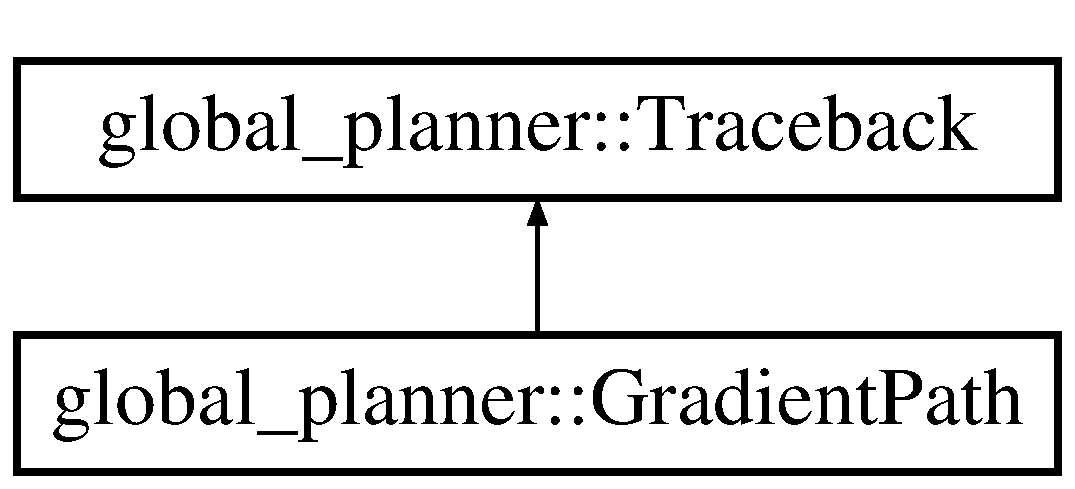
\includegraphics[height=2.000000cm]{classglobal__planner_1_1_gradient_path}
\end{center}
\end{figure}
\subsection*{Public Member Functions}
\begin{DoxyCompactItemize}
\item 
\mbox{\Hypertarget{classglobal__planner_1_1_gradient_path_a57de63c14757b1f84ede9cefac3c3902}\label{classglobal__planner_1_1_gradient_path_a57de63c14757b1f84ede9cefac3c3902}} 
{\bfseries Gradient\+Path} (\mbox{\hyperlink{classglobal__planner_1_1_potential_calculator}{Potential\+Calculator}} $\ast$p\+\_\+calc)
\item 
\mbox{\Hypertarget{classglobal__planner_1_1_gradient_path_a58c7221bd0f4891a218403206953c0b4}\label{classglobal__planner_1_1_gradient_path_a58c7221bd0f4891a218403206953c0b4}} 
void {\bfseries set\+Size} (int xs, int ys)
\item 
\mbox{\Hypertarget{classglobal__planner_1_1_gradient_path_a740775a18f446f585017e7051850a8bf}\label{classglobal__planner_1_1_gradient_path_a740775a18f446f585017e7051850a8bf}} 
bool {\bfseries get\+Path} (float $\ast$potential, double start\+\_\+x, double start\+\_\+y, double end\+\_\+x, double end\+\_\+y, std\+::vector$<$ std\+::pair$<$ float, float $>$ $>$ \&path)
\end{DoxyCompactItemize}
\subsection*{Additional Inherited Members}


The documentation for this class was generated from the following files\+:\begin{DoxyCompactItemize}
\item 
include/global\+\_\+planner/gradient\+\_\+path.\+h\item 
src/gradient\+\_\+path.\+cpp\end{DoxyCompactItemize}

\hypertarget{structglobal__planner_1_1greater1}{}\section{global\+\_\+planner\+:\+:greater1 Struct Reference}
\label{structglobal__planner_1_1greater1}\index{global\+\_\+planner\+::greater1@{global\+\_\+planner\+::greater1}}
\subsection*{Public Member Functions}
\begin{DoxyCompactItemize}
\item 
\mbox{\Hypertarget{structglobal__planner_1_1greater1_a8efdd33231191d4b1178fa16f49eaf17}\label{structglobal__planner_1_1greater1_a8efdd33231191d4b1178fa16f49eaf17}} 
bool {\bfseries operator()} (const \mbox{\hyperlink{classglobal__planner_1_1_index}{Index}} \&a, const \mbox{\hyperlink{classglobal__planner_1_1_index}{Index}} \&b) const
\end{DoxyCompactItemize}


The documentation for this struct was generated from the following file\+:\begin{DoxyCompactItemize}
\item 
include/global\+\_\+planner/astar.\+h\end{DoxyCompactItemize}

\hypertarget{classglobal__planner_1_1_grid_path}{}\section{global\+\_\+planner\+:\+:Grid\+Path Class Reference}
\label{classglobal__planner_1_1_grid_path}\index{global\+\_\+planner\+::\+Grid\+Path@{global\+\_\+planner\+::\+Grid\+Path}}
Inheritance diagram for global\+\_\+planner\+:\+:Grid\+Path\+:\begin{figure}[H]
\begin{center}
\leavevmode
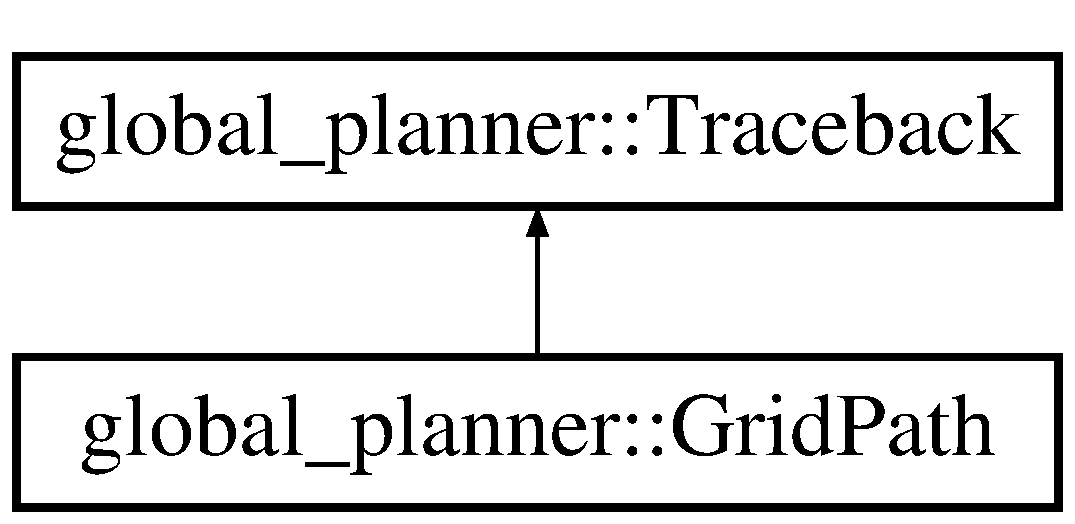
\includegraphics[height=2.000000cm]{classglobal__planner_1_1_grid_path}
\end{center}
\end{figure}
\subsection*{Public Member Functions}
\begin{DoxyCompactItemize}
\item 
\mbox{\Hypertarget{classglobal__planner_1_1_grid_path_ad4b6453a13dc23b79e684e9e2092c25c}\label{classglobal__planner_1_1_grid_path_ad4b6453a13dc23b79e684e9e2092c25c}} 
{\bfseries Grid\+Path} (\mbox{\hyperlink{classglobal__planner_1_1_potential_calculator}{Potential\+Calculator}} $\ast$p\+\_\+calc)
\item 
\mbox{\Hypertarget{classglobal__planner_1_1_grid_path_a11f2838b30fdaca0e29ccff49d0e6c58}\label{classglobal__planner_1_1_grid_path_a11f2838b30fdaca0e29ccff49d0e6c58}} 
bool {\bfseries get\+Path} (float $\ast$potential, double start\+\_\+x, double start\+\_\+y, double end\+\_\+x, double end\+\_\+y, std\+::vector$<$ std\+::pair$<$ float, float $>$ $>$ \&path)
\end{DoxyCompactItemize}
\subsection*{Additional Inherited Members}


The documentation for this class was generated from the following files\+:\begin{DoxyCompactItemize}
\item 
include/global\+\_\+planner/grid\+\_\+path.\+h\item 
src/grid\+\_\+path.\+cpp\end{DoxyCompactItemize}

\hypertarget{classglobal__planner_1_1_index}{}\section{global\+\_\+planner\+:\+:Index Class Reference}
\label{classglobal__planner_1_1_index}\index{global\+\_\+planner\+::\+Index@{global\+\_\+planner\+::\+Index}}
\subsection*{Public Member Functions}
\begin{DoxyCompactItemize}
\item 
\mbox{\Hypertarget{classglobal__planner_1_1_index_a52b5549609f2fbdf06a5e47b3b335492}\label{classglobal__planner_1_1_index_a52b5549609f2fbdf06a5e47b3b335492}} 
{\bfseries Index} (int a, float b)
\end{DoxyCompactItemize}
\subsection*{Public Attributes}
\begin{DoxyCompactItemize}
\item 
\mbox{\Hypertarget{classglobal__planner_1_1_index_a5eaa92e0b2baa2b4e5b93ff2c5ad2514}\label{classglobal__planner_1_1_index_a5eaa92e0b2baa2b4e5b93ff2c5ad2514}} 
int {\bfseries i}
\item 
\mbox{\Hypertarget{classglobal__planner_1_1_index_a014931e74c546a0315feeb4c619f7ee1}\label{classglobal__planner_1_1_index_a014931e74c546a0315feeb4c619f7ee1}} 
float {\bfseries cost}
\end{DoxyCompactItemize}


The documentation for this class was generated from the following file\+:\begin{DoxyCompactItemize}
\item 
include/global\+\_\+planner/astar.\+h\end{DoxyCompactItemize}

\hypertarget{classglobal__planner_1_1_orientation_filter}{}\section{global\+\_\+planner\+:\+:Orientation\+Filter Class Reference}
\label{classglobal__planner_1_1_orientation_filter}\index{global\+\_\+planner\+::\+Orientation\+Filter@{global\+\_\+planner\+::\+Orientation\+Filter}}
\subsection*{Public Member Functions}
\begin{DoxyCompactItemize}
\item 
\mbox{\Hypertarget{classglobal__planner_1_1_orientation_filter_a90c8cd6c44018145bf0ae3e71580c1b1}\label{classglobal__planner_1_1_orientation_filter_a90c8cd6c44018145bf0ae3e71580c1b1}} 
virtual void {\bfseries process\+Path} (const geometry\+\_\+msgs\+::\+Pose\+Stamped \&start, std\+::vector$<$ geometry\+\_\+msgs\+::\+Pose\+Stamped $>$ \&path)
\item 
\mbox{\Hypertarget{classglobal__planner_1_1_orientation_filter_a59770ba7f30c0e87e62b407bc44feda1}\label{classglobal__planner_1_1_orientation_filter_a59770ba7f30c0e87e62b407bc44feda1}} 
void {\bfseries set\+Angle\+Based\+On\+Position\+Derivative} (std\+::vector$<$ geometry\+\_\+msgs\+::\+Pose\+Stamped $>$ \&path, int index)
\item 
\mbox{\Hypertarget{classglobal__planner_1_1_orientation_filter_a36817535ca10c2662b6cc2d0919576bf}\label{classglobal__planner_1_1_orientation_filter_a36817535ca10c2662b6cc2d0919576bf}} 
void {\bfseries interpolate} (std\+::vector$<$ geometry\+\_\+msgs\+::\+Pose\+Stamped $>$ \&path, int start\+\_\+index, int end\+\_\+index)
\item 
\mbox{\Hypertarget{classglobal__planner_1_1_orientation_filter_a1934b57509ac8d2074695bee82c8e178}\label{classglobal__planner_1_1_orientation_filter_a1934b57509ac8d2074695bee82c8e178}} 
void {\bfseries set\+Mode} (Orientation\+Mode new\+\_\+mode)
\item 
\mbox{\Hypertarget{classglobal__planner_1_1_orientation_filter_a7419925acb4ebb8b67bf1ae95f9c4333}\label{classglobal__planner_1_1_orientation_filter_a7419925acb4ebb8b67bf1ae95f9c4333}} 
void {\bfseries set\+Mode} (int new\+\_\+mode)
\item 
\mbox{\Hypertarget{classglobal__planner_1_1_orientation_filter_acf2026f87791f87970220d7a42e42422}\label{classglobal__planner_1_1_orientation_filter_acf2026f87791f87970220d7a42e42422}} 
void {\bfseries set\+Window\+Size} (size\+\_\+t window\+\_\+size)
\end{DoxyCompactItemize}
\subsection*{Protected Attributes}
\begin{DoxyCompactItemize}
\item 
\mbox{\Hypertarget{classglobal__planner_1_1_orientation_filter_a5f155f74ab99402aaaee9f23d8a5741c}\label{classglobal__planner_1_1_orientation_filter_a5f155f74ab99402aaaee9f23d8a5741c}} 
Orientation\+Mode {\bfseries omode\+\_\+}
\item 
\mbox{\Hypertarget{classglobal__planner_1_1_orientation_filter_aed9456a588e42436e590db2a4f0c98dc}\label{classglobal__planner_1_1_orientation_filter_aed9456a588e42436e590db2a4f0c98dc}} 
int {\bfseries window\+\_\+size\+\_\+}
\end{DoxyCompactItemize}


The documentation for this class was generated from the following files\+:\begin{DoxyCompactItemize}
\item 
include/global\+\_\+planner/orientation\+\_\+filter.\+h\item 
src/orientation\+\_\+filter.\+cpp\end{DoxyCompactItemize}

\hypertarget{class_planner_core}{}\section{Planner\+Core Class Reference}
\label{class_planner_core}\index{Planner\+Core@{Planner\+Core}}


Provides a R\+OS wrapper for the global\+\_\+planner planner which runs a fast, interpolated navigation function on a costmap.  




{\ttfamily \#include $<$planner\+\_\+core.\+h$>$}



\subsection{Detailed Description}
Provides a R\+OS wrapper for the global\+\_\+planner planner which runs a fast, interpolated navigation function on a costmap. 

The documentation for this class was generated from the following file\+:\begin{DoxyCompactItemize}
\item 
include/global\+\_\+planner/planner\+\_\+core.\+h\end{DoxyCompactItemize}

\hypertarget{classglobal__planner_1_1_planner_with_costmap}{}\section{global\+\_\+planner\+:\+:Planner\+With\+Costmap Class Reference}
\label{classglobal__planner_1_1_planner_with_costmap}\index{global\+\_\+planner\+::\+Planner\+With\+Costmap@{global\+\_\+planner\+::\+Planner\+With\+Costmap}}
Inheritance diagram for global\+\_\+planner\+:\+:Planner\+With\+Costmap\+:\begin{figure}[H]
\begin{center}
\leavevmode
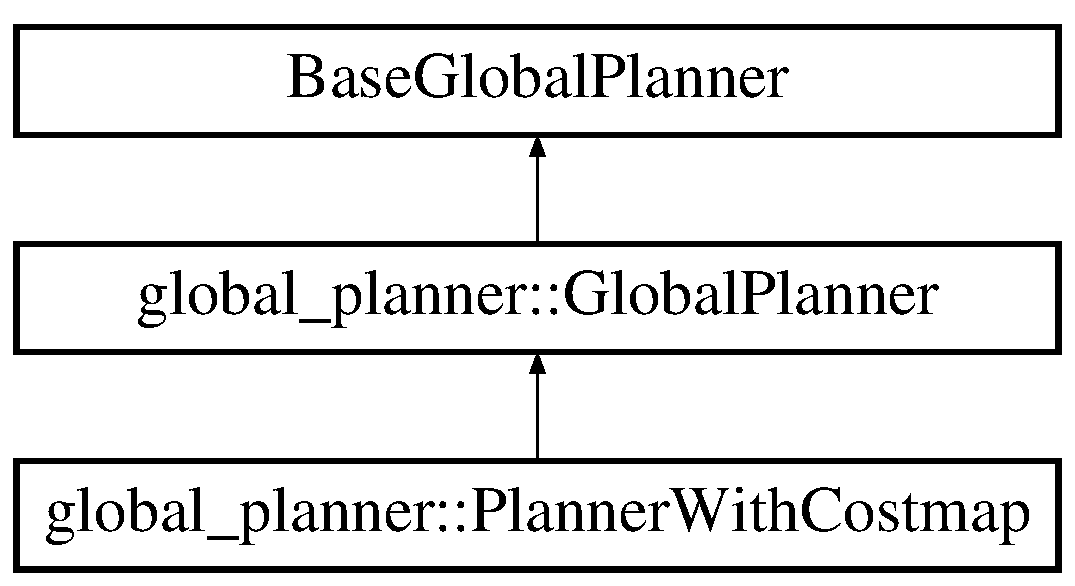
\includegraphics[height=3.000000cm]{classglobal__planner_1_1_planner_with_costmap}
\end{center}
\end{figure}
\subsection*{Public Member Functions}
\begin{DoxyCompactItemize}
\item 
\mbox{\Hypertarget{classglobal__planner_1_1_planner_with_costmap_abf6efea3cec2f9f41ae7104005f777c7}\label{classglobal__planner_1_1_planner_with_costmap_abf6efea3cec2f9f41ae7104005f777c7}} 
{\bfseries Planner\+With\+Costmap} (string name, Costmap2\+D\+R\+OS $\ast$cmap)
\item 
\mbox{\Hypertarget{classglobal__planner_1_1_planner_with_costmap_a735f4750a1e88ab01b22a4d12d8dfc0d}\label{classglobal__planner_1_1_planner_with_costmap_a735f4750a1e88ab01b22a4d12d8dfc0d}} 
bool {\bfseries make\+Plan\+Service} (navfn\+::\+Make\+Nav\+Plan\+::\+Request \&req, navfn\+::\+Make\+Nav\+Plan\+::\+Response \&resp)
\end{DoxyCompactItemize}
\subsection*{Additional Inherited Members}


The documentation for this class was generated from the following file\+:\begin{DoxyCompactItemize}
\item 
src/plan\+\_\+node.\+cpp\end{DoxyCompactItemize}

\hypertarget{classglobal__planner_1_1_potential_calculator}{}\section{global\+\_\+planner\+:\+:Potential\+Calculator Class Reference}
\label{classglobal__planner_1_1_potential_calculator}\index{global\+\_\+planner\+::\+Potential\+Calculator@{global\+\_\+planner\+::\+Potential\+Calculator}}
Inheritance diagram for global\+\_\+planner\+:\+:Potential\+Calculator\+:\begin{figure}[H]
\begin{center}
\leavevmode
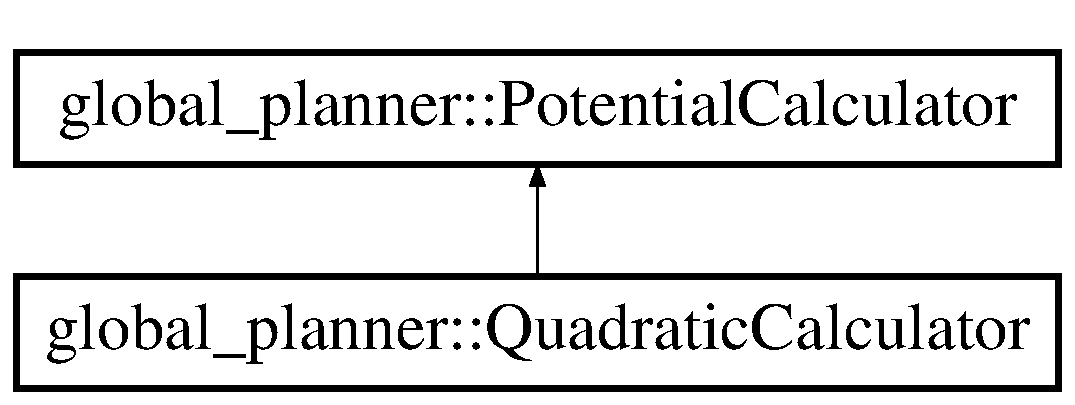
\includegraphics[height=2.000000cm]{classglobal__planner_1_1_potential_calculator}
\end{center}
\end{figure}
\subsection*{Public Member Functions}
\begin{DoxyCompactItemize}
\item 
\mbox{\Hypertarget{classglobal__planner_1_1_potential_calculator_a9e785461ad18ae3e6a393dedcf903a6a}\label{classglobal__planner_1_1_potential_calculator_a9e785461ad18ae3e6a393dedcf903a6a}} 
{\bfseries Potential\+Calculator} (int nx, int ny)
\item 
\mbox{\Hypertarget{classglobal__planner_1_1_potential_calculator_a4befc4819934603d43c8dc539f445fd4}\label{classglobal__planner_1_1_potential_calculator_a4befc4819934603d43c8dc539f445fd4}} 
virtual float {\bfseries calculate\+Potential} (float $\ast$potential, unsigned char cost, int n, float prev\+\_\+potential=-\/1)
\item 
virtual void \mbox{\hyperlink{classglobal__planner_1_1_potential_calculator_a9ff19259198704723eb62d515ea91e58}{set\+Size}} (int nx, int ny)
\begin{DoxyCompactList}\small\item\em Sets or resets the size of the map. \end{DoxyCompactList}\end{DoxyCompactItemize}
\subsection*{Protected Member Functions}
\begin{DoxyCompactItemize}
\item 
\mbox{\Hypertarget{classglobal__planner_1_1_potential_calculator_a82306cd4356d50c5f9a11b22c7668202}\label{classglobal__planner_1_1_potential_calculator_a82306cd4356d50c5f9a11b22c7668202}} 
int {\bfseries to\+Index} (int x, int y)
\end{DoxyCompactItemize}
\subsection*{Protected Attributes}
\begin{DoxyCompactItemize}
\item 
\mbox{\Hypertarget{classglobal__planner_1_1_potential_calculator_ad5102b7868d243fef672bbe772571339}\label{classglobal__planner_1_1_potential_calculator_ad5102b7868d243fef672bbe772571339}} 
int {\bfseries nx\+\_\+}
\item 
\mbox{\Hypertarget{classglobal__planner_1_1_potential_calculator_a2f6e7eb5facdf52141299329b546e745}\label{classglobal__planner_1_1_potential_calculator_a2f6e7eb5facdf52141299329b546e745}} 
int {\bfseries ny\+\_\+}
\item 
int \mbox{\hyperlink{classglobal__planner_1_1_potential_calculator_a5c62eff3a3c95db6cd6dedcb9cfb3e2a}{ns\+\_\+}}
\end{DoxyCompactItemize}


\subsection{Member Function Documentation}
\mbox{\Hypertarget{classglobal__planner_1_1_potential_calculator_a9ff19259198704723eb62d515ea91e58}\label{classglobal__planner_1_1_potential_calculator_a9ff19259198704723eb62d515ea91e58}} 
\index{global\+\_\+planner\+::\+Potential\+Calculator@{global\+\_\+planner\+::\+Potential\+Calculator}!set\+Size@{set\+Size}}
\index{set\+Size@{set\+Size}!global\+\_\+planner\+::\+Potential\+Calculator@{global\+\_\+planner\+::\+Potential\+Calculator}}
\subsubsection{\texorpdfstring{set\+Size()}{setSize()}}
{\footnotesize\ttfamily virtual void global\+\_\+planner\+::\+Potential\+Calculator\+::set\+Size (\begin{DoxyParamCaption}\item[{int}]{nx,  }\item[{int}]{ny }\end{DoxyParamCaption})\hspace{0.3cm}{\ttfamily [inline]}, {\ttfamily [virtual]}}



Sets or resets the size of the map. 


\begin{DoxyParams}{Parameters}
{\em nx} & The x size of the map \\
\hline
{\em ny} & The y size of the mapsets or resets the size of the map \\
\hline
\end{DoxyParams}


\subsection{Member Data Documentation}
\mbox{\Hypertarget{classglobal__planner_1_1_potential_calculator_a5c62eff3a3c95db6cd6dedcb9cfb3e2a}\label{classglobal__planner_1_1_potential_calculator_a5c62eff3a3c95db6cd6dedcb9cfb3e2a}} 
\index{global\+\_\+planner\+::\+Potential\+Calculator@{global\+\_\+planner\+::\+Potential\+Calculator}!ns\+\_\+@{ns\+\_\+}}
\index{ns\+\_\+@{ns\+\_\+}!global\+\_\+planner\+::\+Potential\+Calculator@{global\+\_\+planner\+::\+Potential\+Calculator}}
\subsubsection{\texorpdfstring{ns\+\_\+}{ns\_}}
{\footnotesize\ttfamily int global\+\_\+planner\+::\+Potential\+Calculator\+::ns\+\_\+\hspace{0.3cm}{\ttfamily [protected]}}

size of grid, in pixels 

The documentation for this class was generated from the following file\+:\begin{DoxyCompactItemize}
\item 
include/global\+\_\+planner/potential\+\_\+calculator.\+h\end{DoxyCompactItemize}

\hypertarget{classglobal__planner_1_1_quadratic_calculator}{}\section{global\+\_\+planner\+:\+:Quadratic\+Calculator Class Reference}
\label{classglobal__planner_1_1_quadratic_calculator}\index{global\+\_\+planner\+::\+Quadratic\+Calculator@{global\+\_\+planner\+::\+Quadratic\+Calculator}}
Inheritance diagram for global\+\_\+planner\+:\+:Quadratic\+Calculator\+:\begin{figure}[H]
\begin{center}
\leavevmode
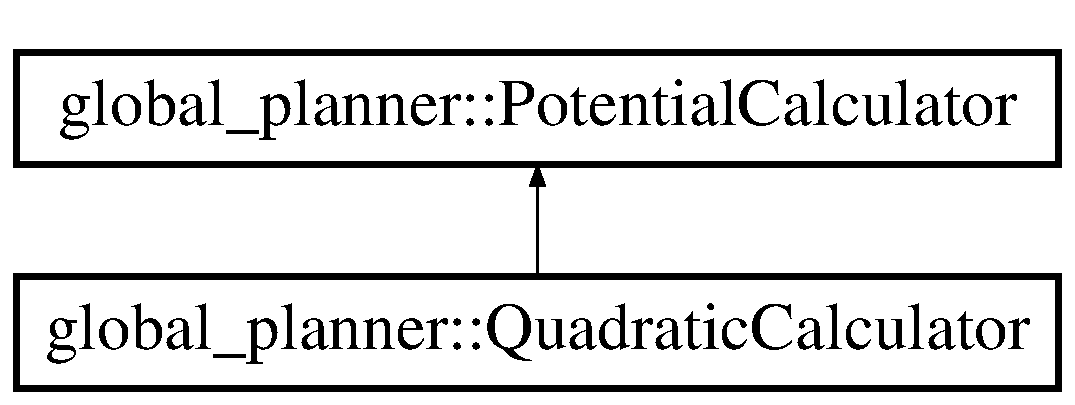
\includegraphics[height=2.000000cm]{classglobal__planner_1_1_quadratic_calculator}
\end{center}
\end{figure}
\subsection*{Public Member Functions}
\begin{DoxyCompactItemize}
\item 
\mbox{\Hypertarget{classglobal__planner_1_1_quadratic_calculator_a4b4e966d382c85d0212121c674587f60}\label{classglobal__planner_1_1_quadratic_calculator_a4b4e966d382c85d0212121c674587f60}} 
{\bfseries Quadratic\+Calculator} (int nx, int ny)
\item 
\mbox{\Hypertarget{classglobal__planner_1_1_quadratic_calculator_a5cb0a0126df397b4b5d86d871ddab1d4}\label{classglobal__planner_1_1_quadratic_calculator_a5cb0a0126df397b4b5d86d871ddab1d4}} 
float {\bfseries calculate\+Potential} (float $\ast$potential, unsigned char cost, int n, float prev\+\_\+potential)
\end{DoxyCompactItemize}
\subsection*{Additional Inherited Members}


The documentation for this class was generated from the following files\+:\begin{DoxyCompactItemize}
\item 
include/global\+\_\+planner/quadratic\+\_\+calculator.\+h\item 
src/quadratic\+\_\+calculator.\+cpp\end{DoxyCompactItemize}

\hypertarget{classglobal__planner_1_1_traceback}{}\section{global\+\_\+planner\+:\+:Traceback Class Reference}
\label{classglobal__planner_1_1_traceback}\index{global\+\_\+planner\+::\+Traceback@{global\+\_\+planner\+::\+Traceback}}
Inheritance diagram for global\+\_\+planner\+:\+:Traceback\+:\begin{figure}[H]
\begin{center}
\leavevmode
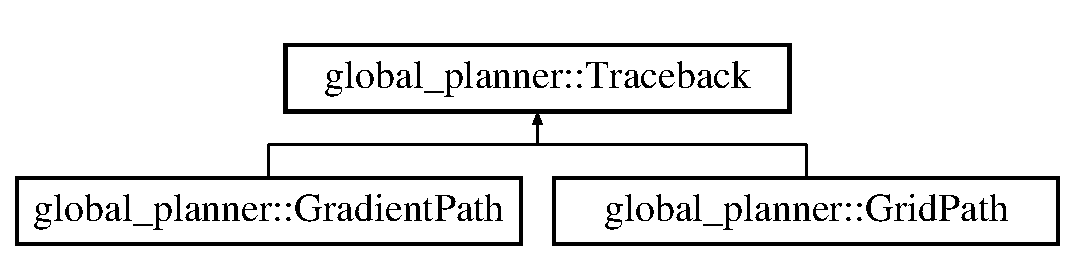
\includegraphics[height=2.000000cm]{classglobal__planner_1_1_traceback}
\end{center}
\end{figure}
\subsection*{Public Member Functions}
\begin{DoxyCompactItemize}
\item 
\mbox{\Hypertarget{classglobal__planner_1_1_traceback_abf48245c8bc021ba9df355ae74ded3e4}\label{classglobal__planner_1_1_traceback_abf48245c8bc021ba9df355ae74ded3e4}} 
{\bfseries Traceback} (\mbox{\hyperlink{classglobal__planner_1_1_potential_calculator}{Potential\+Calculator}} $\ast$p\+\_\+calc)
\item 
\mbox{\Hypertarget{classglobal__planner_1_1_traceback_ad3562c3ff5dc3a1e4465d2ddbe62f812}\label{classglobal__planner_1_1_traceback_ad3562c3ff5dc3a1e4465d2ddbe62f812}} 
virtual bool {\bfseries get\+Path} (float $\ast$potential, double start\+\_\+x, double start\+\_\+y, double end\+\_\+x, double end\+\_\+y, std\+::vector$<$ std\+::pair$<$ float, float $>$ $>$ \&path)=0
\item 
\mbox{\Hypertarget{classglobal__planner_1_1_traceback_a75fa8c3628baa7debd94ac83b02e03a7}\label{classglobal__planner_1_1_traceback_a75fa8c3628baa7debd94ac83b02e03a7}} 
virtual void {\bfseries set\+Size} (int xs, int ys)
\item 
\mbox{\Hypertarget{classglobal__planner_1_1_traceback_a9565bfa976f8ce019ce4e4d814b3b575}\label{classglobal__planner_1_1_traceback_a9565bfa976f8ce019ce4e4d814b3b575}} 
int {\bfseries get\+Index} (int x, int y)
\item 
\mbox{\Hypertarget{classglobal__planner_1_1_traceback_af411eb96102bcedea2d530137b13a002}\label{classglobal__planner_1_1_traceback_af411eb96102bcedea2d530137b13a002}} 
void {\bfseries set\+Lethal\+Cost} (unsigned char lethal\+\_\+cost)
\end{DoxyCompactItemize}
\subsection*{Protected Attributes}
\begin{DoxyCompactItemize}
\item 
\mbox{\Hypertarget{classglobal__planner_1_1_traceback_a062d8297437fb132a87a9adff70c2c8f}\label{classglobal__planner_1_1_traceback_a062d8297437fb132a87a9adff70c2c8f}} 
int {\bfseries xs\+\_\+}
\item 
\mbox{\Hypertarget{classglobal__planner_1_1_traceback_a1d7c2fd48b6d48696ee7fcd650e5cc4b}\label{classglobal__planner_1_1_traceback_a1d7c2fd48b6d48696ee7fcd650e5cc4b}} 
int {\bfseries ys\+\_\+}
\item 
\mbox{\Hypertarget{classglobal__planner_1_1_traceback_a61b0a5a5dfb61d942d2dfd7c0d7a58ea}\label{classglobal__planner_1_1_traceback_a61b0a5a5dfb61d942d2dfd7c0d7a58ea}} 
unsigned char {\bfseries lethal\+\_\+cost\+\_\+}
\item 
\mbox{\Hypertarget{classglobal__planner_1_1_traceback_a918825f1ecb2858a3b4a6d516ad144b4}\label{classglobal__planner_1_1_traceback_a918825f1ecb2858a3b4a6d516ad144b4}} 
\mbox{\hyperlink{classglobal__planner_1_1_potential_calculator}{Potential\+Calculator}} $\ast$ {\bfseries p\+\_\+calc\+\_\+}
\end{DoxyCompactItemize}


The documentation for this class was generated from the following file\+:\begin{DoxyCompactItemize}
\item 
include/global\+\_\+planner/traceback.\+h\end{DoxyCompactItemize}

%--- End generated contents ---

% Index
\backmatter
\newpage
\phantomsection
\clearemptydoublepage
\addcontentsline{toc}{chapter}{Index}
\printindex

\end{document}
